\subsubsection{Testo}
Il testo è disposto orizzontalmente (non per colonne) in brevi paragrafi, in
alcuni casi la disposizione dei contenuti è in forma di lista ed in rari casi 
in forma di liste affiancate. Per quest'ultima opzione le informazioni 
dovrebbero essere più strutturate (i.e. brevi sottosezioni come accennato in
\ref{overview}) altrimenti l'utente è affaticato nella ricerca all'interno
 di una struttura così complicata. 
\begin{figure}[ht]
\centering
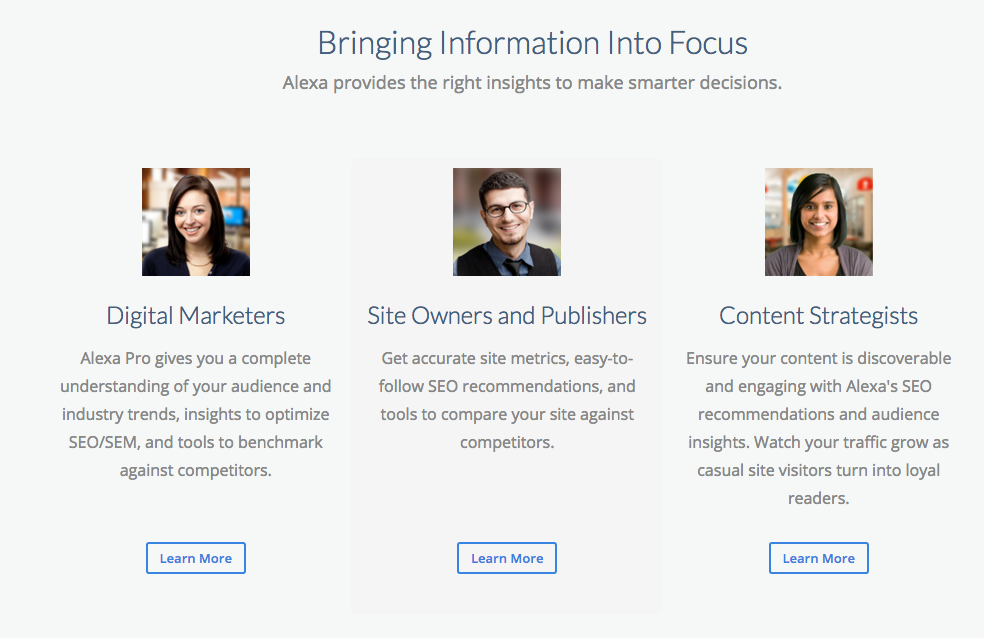
\includegraphics[scale=0.30,keepaspectratio]{{figure/4/blurb0}.png}
\caption{Esempio di titolo con blurb}
\end{figure}
\FloatBarrier 
Ad ogni titolo di paragrafo è associato
 un breve blurb per fornire le informazioni chiave che questo contiene.\\
Risultato : \textit{8.5}